\begin{frame}{Konstrukcija pravokotnice na premico $p$ skozi točko $T$}

\begin{columns}
	
	\begin{column}{0.55\textwidth}
			\begin{itemize}[<+->]
			 \item Dani sta premica $p$ in točka $T$.
			 \item Nariši lok $k$ s središčem v $T$.
			 \item Premico $p$ seče v točkah $A$ in $B$.
			 \item Nariši lok $m$ s središčem v $A$.
			 \item Nariši lok $n$ s središčem v $B$ in z enakim polmerom.
			 \item Loka se sečeta v točki $C$.
			 \item Premica skozi točki $T$ in $C$ je pravokotna na $p$.
		  \end{itemize}
	\end{column}
		
	\begin{column}{0.45\textwidth}
		  \vfill
		  \only<1>{\includegraphics[width=1\textwidth]{slike/fig-1.png}}
		  % \only<2>{\includegraphics[width=1\textwidth]{slike/fig-2.png}}
		  % \only<3>{\includegraphics[width=1\textwidth]{slike/fig-3.png}}
		  % \only<4>{\includegraphics[width=1\textwidth]{slike/fig-4.png}}
		  % \only<5>{\includegraphics[width=1\textwidth]{slike/fig-5.png}}
		  % \only<6>{\includegraphics[width=1\textwidth]{slike/fig-6.png}}
		  % \only<7>{\includegraphics[width=1\textwidth]{slike/fig-7.png}}
	\end{column}

\end{columns}

\end{frame}

\begin{frame}{Konstrukcija pravokotnice na premico $p$ skozi točko $T$}

\begin{columns}
	
	\begin{column}{0.55\textwidth}
			\begin{itemize}[<+->]
			 \item Dani sta premica $p$ in točka $T$.
			 \item Nariši lok $k$ s središčem v $T$.
			 \item Premico $p$ seče v točkah $A$ in $B$.
			 \item Nariši lok $m$ s središčem v $A$.
			 \item Nariši lok $n$ s središčem v $B$ in z enakim polmerom.
			 \item Loka se sečeta v točki $C$.
			 \item Premica skozi točki $T$ in $C$ je pravokotna na $p$.
		  \end{itemize}
	\end{column}
		
	\begin{column}{0.45\textwidth}
		  \vfill
		  \begin{tikzpicture}
			% % Sliko smo naredili tako, da so točke A, B, T in C vse enako oddaljene
				% % od presečišča premic; kot ATC je 45°.
				% % Vsi krožni loki imajo radij 2.
				\tikzmath{
				% 	% Razdalja od točke T do premice p je tako 2*sin(45°).
					\t = 2*sin(45);
				% 	% Razdalja začetka loka m do premice p
				% 	% oz. razdalja točke T' levo in zgoraj od točke T do premice
					\tt = 2*sin(60);
				% 	% Razdalja točke T' od navpične premice skozi T
					\td = \t-2*cos(60);
				}
				% % Definicija točke T
				\coordinate [label={[blue, above left]:$T$}] (T) at (0,{\t});
				% % Risanje točke T
				\fill[blue] (T) circle (2pt);
				% % Premica p
				\draw[blue, very thick] (-2,0) -- (2,0) node[right] {$p$};
				\pause
				% % Definicija pomožne točke A' in risanje krožnega loka k, ki se začne v A'
				\coordinate (A') at ({-\tt},{\td});
				\draw[gray, thin] (A') arc[start angle=210, end angle=330, radius=2] node[right] {\scriptsize $k$};
				\pause
				% % Točka A
				\coordinate [label=below left:{\scriptsize $A$}] (A) at ({-\t},0);
				\draw (A) circle (1.5pt);
				
				% % Naloga 3.4.1.: Narišite še točko B (skupaj z oznako)
				\coordinate [label=below right:{\scriptsize $B$}] (B) at ({\t},0);
				\fill<5->[red] (B) circle (2pt);
				
				% % Naloga 3.4.2.: Definirajte točko T', v kateri se začne lok m in narišite lok m z oznako.
				% % Lok je definiran s točko, v kateri se lok začne (ne središče!), z začetnim in končnim kotom ter radijem.
				% % Koti so vedno podani enako: kot 0 je v smeri x osi in se veča v nasprotni smeri urinega kazalca.
				\coordinate (Tprime) at ({-1},{1.5});
				\draw<6->[gray, thin] (Tprime) arc[start angle=0, end angle=90, radius=2] node[right]{\scriptsize $m$};

				% % Naloga 3.4.3.: Definirajte točko T'' in narišite lok n z oznako.
				\coordinate (Tdoubleprime) at ({1},{1.5});
				\draw<7->[gray, thin] (Tdoubleprime) arc[start angle=90, end angle=180, radius=2] node[left]{\scriptsize $n$};
				% % Naloga 3.4.4.: Definirajte in narišite točko C.
				\coordinate [label=above right:{\scriptsize $C$}] (C) at (0,2);
				\fill<8->[green] (C) circle (2pt);

				% % Naloga 3.4.5.: Narišite premico skozi točki T in C.	
				\draw<9->[blue, thick] (T) -- (C);
		  \end{tikzpicture}
	\end{column}

\end{columns}

\end{frame}
         

% Naloga 4
 \begin{frame}{Graf funkcije s TikZ}
 	\centering
 	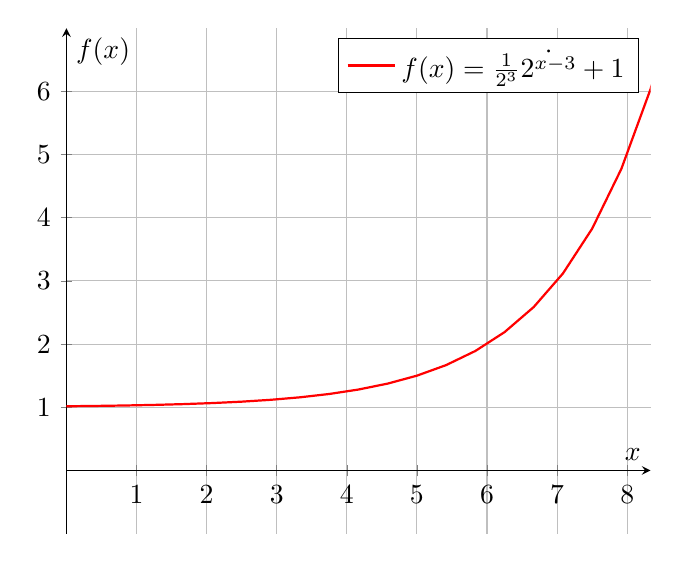
\begin{tikzpicture}
 		\begin{axis}[
 			axis lines = middle,
 			domain = 0:10,
 			width = 9cm,
 			height = 8cm,
 			xtick = {0, 1, 2, 3, 4, 5, 6, 7, 8},
 			ytick = {0, 1, 2, 3, 4, 5, 6},
 			ymin = -1,
 			ymax = 7,
 			grid = both,
			xlabel = {$x$},
			ylabel = {$f(x)$}
 		]
			\addplot[thick, red] {2^(x-3)/8 + 1};
			\addlegendentry{$f(x) = \frac{1}{2^3}\dot{2^{x-3}} + 1$}
 		\end{axis}
 	\end{tikzpicture}
 \end{frame}